%%% 陆亚明老师编写的《数学分析入门》的排版方式 %%%

\documentclass[11pt,twoside,a4paper]{book}

\usepackage[UTF8,heading = true]{ctex}
\usepackage{geometry,graphicx,xcolor,color}
\usepackage{amssymb,amsmath,amsthm}        % 数学字体
\usepackage{newpxtext,mathpazo}            % 采用 Palatino 风格字体
\usepackage{newclude,ulem}
\usepackage{float} %设置图片浮动位置的宏包
\usepackage{subfigure} %插入多图时用子图显示的宏包

\definecolor{winered}{rgb}{0.5,0,0}
\definecolor{structurecolor}{RGB}{122,122,142}
\definecolor{main}{rgb}{0.5,0,0}
\definecolor{second}{RGB}{115,45,2}
\definecolor{third}{RGB}{0,80,80}
\usepackage[colorlinks,linkcolor = winered]{hyperref}    % 定义引用的颜色


%%%%%%%%%%%%%%% 定义定理环境 %%%%%%%%%%%%%%%%%%%
\newtheoremstyle{defstyle}{3pt}{3pt}{\kaishu}{-3pt}{
  \bfseries\color{main}}{}{0.5em}{\indent 【\thmname{#1} \thmnumber{#2}】 \thmnote{(#3)}}
\newtheoremstyle{thmstyle}{3pt}{3pt}{\kaishu}{-3pt}{
  \bfseries\color{second}}{}{0.5em}{\indent【\thmname{#1} \thmnumber{#2}】 \thmnote{(#3)}}
\newtheoremstyle{prostyle}{3pt}{3pt}{\kaishu}{-3pt}{
  \bfseries\color{third}}{}{0.5em}{\indent【\thmname{#1} \thmnumber{#2}】 \thmnote{(#3)}}

\theoremstyle{thmstyle} %theorem style
  \newtheorem{theorem}{定理}[chapter]
\theoremstyle{defstyle} % definition style
  \newtheorem{definition}[theorem]{定义}
  \newtheorem{lemma}[theorem]{引理}
  \newtheorem{corollary}[theorem]{推论}
\theoremstyle{prostyle} % proposition style
  \newtheorem{proposition}[theorem]{命题}
  \newtheorem{example}[theorem]{例题}

\renewenvironment{proof}[1][证明]{\par{\kaishu \uline{\textbf{#1.}}} \;\fangsong}{\qed\par}
\newenvironment{solution}{\par\underline{\textbf{解.}} \;\kaishu}{\par}
\newenvironment{remark}{\par\underline{\textbf{注.}} \;\fangsong}{\par}
\newcommand{\intro}[1]{\rightline{\parbox[t]{5cm}{\footnotesize \fangsong\quad\quad #1 }}}
% ------------------------------------------------------------%

\usepackage{enumerate}
\usepackage{enumitem}
\setlist[enumerate,1]{label=\color{structurecolor}\arabic*.}
\setlist[enumerate,2]{label=\color{structurecolor}(\arabic*).}
\setlist[enumerate,3]{label=\color{structurecolor}\Roman*.}
\setlist[enumerate,4]{label=\color{structurecolor}\Alph*.}

%%%%%%%%%%%%%%%%%%%%%% 设置章形式 %%%%%%%%%%%%%%%%%%%%%%%%%%%%%
% \setlength{\parindent}{0pt}  % 设置段首缩进	
\usepackage{titlesec,titletoc}  % 设置标题格式, 定制目录列表样式

\linespread{1.5}

\usepackage{fancyhdr}
\fancypagestyle{plain}{
% \fancyhf{} % clear all header and footer fields
\fancyhead{} %  页眉清空
\renewcommand{\headrulewidth}{0pt} % 去页眉线
\renewcommand{\footrulewidth}{0pt}
}

\titlecontents{chapter}[0em]{}{\large \fangsong{第 \thecontentslabel 章\quad}}{}{\hfill\contentspage}
\titlecontents{section}[2em]{}{\thecontentslabel\quad\textcolor{blue}}{}{\titlerule*{ .} \contentspage}

\titleformat{\chapter}[display]{\Large}
	{\color{structurecolor}\centering\small \color{structurecolor}第 \zhnumber{\arabic{chapter}} \ 章 }{0.5ex}
	{\color{structurecolor}{\titlerule[1pt]}\Large \kaishu \centering \bfseries}

%\titleformat{\chapter}{\centering\Huge\bfseries}{第\,\thechapter\,章}{1em}{}
%\titleformat{\section}{\raggedright\Large\bfseries}{\,\thesection\,}{1em}{}
%\titleformat{\subsection}{\raggedright\large\bfseries}{\,\thesubsection\,}{1em}{}

%\ctexset{chapter = {
%  name = {第,章},
%  number = \chinese{chapter},
%  nameformat = \Huge \heiti \centering \bfseries,
%  titleformat = \Huge \heiti \centering \bfseries,
%  }
%}

\titleformat{\section}[frame]
{\normalfont\color{structurecolor}}
    {\footnotesize \enspace \large \textcolor{structurecolor}{\S \,\thesection}\enspace}{10pt}
    {\Large\filcenter \bf \kaishu }

\titlespacing*{\section}{1pc}{*7}{*2.3}[1pc]
\titleformat{\subsection}[hang]{\bfseries}{
    \large\bfseries\color{structurecolor}\thesubsection\enspace}{1pt}{%
    \color{structurecolor}\large\bfseries\filright}
\titleformat{\subsubsection}[hang]{\bfseries}{
    \large\bfseries\color{structurecolor}\thesubsubsection\enspace}{1pt}{%
    \color{structurecolor}\large\bfseries\filright}

\title{《数学分析入门》的排版方式}
\author{李四杰}
\date{\today}

\begin{document}

\maketitle

\newpage

\tableofcontents
\thispagestyle{empty}

\newpage
\setcounter{page}{1}
\chapter{集合与映射}

\intro{
    在数学中,严格性不是一切,但是没有它便没有一切。不严格的证明微不足道。

    \rightline{——H.Poincar$\mathrm{\acute{e}}$}
}

\section{集合}

    \begin{definition}
        设\(A, B\)是两个集合,若\(A\)中元素均属于\(B\),则称\(A\)为\(B\)的\uline{子集},记作\(A \subseteq B\)或者\(B \supseteq A\)。此时也称\uline{\(A\)包含于\(B\)},或\uline{\(B\)包含于\(A\)}。若\(A \subseteq B\)且存在\(B\)中的元素不属于\(A\),则称\(A\)为\(B\)的\uline{真子集},记作\(A \subset B\)或者\( B \supset A\)。
    \end{definition}

    \begin{theorem}
    abcdefg.
    \end{theorem}

    \begin{proposition}
        \(( a, b) = (c, d)\)当且仅当\(a = c\) 且\(b = d\)。
    \end{proposition}

    \begin{proof}
        充分性是显然的。下证明必要性。如果\((a, b) = (c, d)\),那么$$\{\{a\}, \{a, b\} = \{\{c\}, \{c, d\}\}$$
        \begin{enumerate}
            \item 若\(a = b\),则有$$\{\{a \}\} = \{\{c\}, \{c, d\}\}$$那么\(c = d\)否则上式右侧有两个元素。
            \item 若\(a \neq b\),则必有\(c \neq d\),否则左侧有两个元素而右侧有一个元素。而且必有$$\{a\} = \{c\} \qquad \text{且}\qquad \{a, b\} = \{ c, d\}$$进而\(a = c\)且\(b = d\)。
        \end{enumerate}
    \end{proof}

    \begin{example}
    求解方程:\(x^2 - 2 x + 1 = 0\).
    \end{example}

    \begin{solution}
    Since \[x^2 - 2 x + 1 = (x - 1)^2 = 0\]
    Then \[x = \{-1,1\}\]
    \end{solution}
    总有一天,总有一天,

人们的良心将会发现:

人民曾经拥有过

那么扬眉吐气的日子。

一个旷古未有的

伟大的民族英雄,

以压倒一切敌人的气概,

洗雪了 1840 年以来的

所有耻辱和悲伤。

从董存瑞到黄继光,

他们证明了:

一切反动派都是纸老虎。

总有一天,

这个国家的的历史将会记载:

人民曾经谱写过

气壮山河的诗篇。

一个农民的儿子,

在一块农业国的土地上,

用社会主义创造了

属于人民的工农业体系。

从钱学森到王进喜,

他们证明了:

社会主义建设者,

第一次把谋生的劳动,

变成了光荣与神圣的使命。

总有一天,

中国的历史学家将会承认:

这个从来不缺少

帝王将相的古国,

曾经拥有一位

真正的人民领袖。

这个被无数敌人咒骂的人

却没有一个私敌,

除了他的思想,

也没有遗产,

但他有一个牺牲者的名单。

从杨开慧到毛岸英......

总有一天

人们会明白,

为什么一个中国人逝世,

世界 53 个国家下半旗,

联合国最快下半旗...

总有一天,总有一天,

人们会明白,为什么

天南海北、

男女老少、

各行各业、

亿万各族人民,

为一个从来都没见过的人逝世

而悲痛欲绝....

老百姓对毛主席的真挚情感

总有一天,总有一天,

人们会明白,为什么这么多年了,

瞻仰遗容的人总是排队长龙,

参观故居的人总是川流不息...

总有一天,总有一天,

人们会明白,为什么

为什么罗瑞卿大将

走出秦城的第一件事,

是来到天安门向领袖像敬礼,

为什么叶帅在 80 年代一听见别人

提起毛泽东的名字或者谈论毛主席,

就激动得老泪纵横甚至

每当人们提起他的名字,嚎啕大哭......

为什么陈毅元帅病重期间,

几个月都靠输液维持生命,

未曾吃进一粒米,

12 月 26 日,他却要求吃面,

看他吃的非常艰难,

护理人员都劝他别吃了,

他费力地说:今天是毛主席生日,我要为他吃长寿面啊!

所有在场人员都感动热泪...

他们跟主席是一种什么样的感情,谁能用语言描述?

总有一天,

人们会明白

为什么亚非拉的朋友感激:

“毛主义” 带给了他们

争取民族独立和自由的勇气。

一个天生蔑视所有强权

并敢于把一切

剥削欺压人民的体系和规则撕碎的革命者,

必然受弱小民族和国家的爱戴。

从越南到古巴,

从格瓦拉到曼德拉,

他们证明了:

哪里有压迫

哪里就有反抗,

就是这个世界上

最彻底的民主宣言。

总有一天,

几千年靠天吃饭的农民

将会记起:

他们曾经组织起来过,

把拜神的诚恐

变成了改天换地的自豪。

八万座水库,

上亿亩大寨田,

就连土得掉渣的社办企业,

日后也成为改革中的异军突起。

一个小农经济的王国,

也曾经有过

农业合作社的欢歌。

总有一天,

这个国家的人民

将会想起:

他们曾经

跟随自己的领袖,

进行过一场

人类历史上

从未有过的探索,

进行过一次

追求平等和世界大同的

理想主义战斗。

从纺织女工郝建秀

到拿工分的农民宰相陈永贵,

他们证明了:

社会主义国家

劳动人民地位就是高。

总有一天,

西点军校的课本终将承认:

不怕人民解放军现代化,

就怕毛泽东化,

这支把支部建在连上,

把官兵平等和

军爱民、民拥军

视为生命的军队,

从上甘岭到珍宝岛,

书写的都是

以弱胜强的传奇

和不朽的军魂。

总有一天,

嫦娥故乡的飞船

将在月球登陆:

是独立自主、

自力更生精神

挺起了中国的脊梁,

于是,新中国拥有

无数的 “第一次”,

消灭了无数的 “不可能”,

也无数次的令西方世界”

刮目相看”。

总有一天,

我们的孩子,

我们的后代

会感概向往长辈们

曾经经历过的那个时代,

会把德、智、体全面发展

作为人生的价值目标取向,

会把” 好好学习、天天向上” 教诲

一代代的传承下去。

总有一天,

共和国的史册

会这样铭记:

他是中华民族有史以来

最伟大最杰出的民族英雄之一,

也是世界共产主义运动中

最卓越最勇敢的领袖之一,

他让他的祖国

拥有了主权与尊严,

他让他的人民

拥有了主人公的荣光,

而他的名字

总是与 “人民”

联系在一起的。

总有一天,

这个党的后代们

会不容置疑的感悟到:

凝聚着先辈们集体智慧结晶的

毛泽东思想,

是颠扑不破的真理,

是引领人类构建

大众政治文明的灯塔

而只有当中国

在这一思想牵引下

博发出民族

强大凝聚与向心力时,

才是我中华巨龙的

真正腾飞之时。

而这一思想的精髓就是

“永远站在大多数人民一边!”

总有那么一天,

我们将代代传颂这个人的名字:

人民领袖毛泽东!

他永远是人民心中不落的红太阳!

中华儿女不会忘记您!

\section{映射}
“事物总是要走向反面的,吹得越高,跌得越重,我是准备跌得粉碎的。那也没有什么要紧,物质不灭,不过粉碎罢了!”

你太高看他们了,他们懂什么是资本主义?最多倒退回半封建半殖民地社会。资本主义是靠侵略和掠夺别的国家而积累资产的,他们敢侵略谁呀?不被侵略就阿弥陀佛喽。

“我要把我的一生写进书里,至于我是个好人还是坏人。交给后人来判断。我这个人,有 70\% 的好,30\% 的坏,我就满足了。” ​

我们有两个大教员: 一个是日本人,一个是委员长。这两个大教员不要薪水给我们上课。没有这两个大教员,就教育不了中国人民,教育不了我们党。至于我们党里面有一些小教员,字也认得不多,也讲不出好多道理,他们去讲人家就不听。后来请了一个日本人,一个中国人,一个是日本法西斯,一个是委员长,这两个教员帮我们一教,就教好了。(1945 年在中共七大上作的口头政治报告)

“我的职位如此之低,以致人们都不屑和我来往。我的工作之一就是登记来馆读报的人名,不过这般人大半都不把我放在眼里。在这许多人名之中,我记得有几个是新文化运动著名的领袖,是我十分景仰的人。我很想和他们讨论关于政治和文化的事情,不过他们都是极忙的人,没有时间来倾听一个南边口音的图书佐理员所讲的话。

1976年6月15日,毛泽东同华国锋等人进行重要谈话。毛泽东在病情加重的情况下,召见华国锋等人,对他们说,人生七十古来稀,我八十多岁了,人老总想后事。中国有句古话叫盖棺定论,我虽未盖棺也快了,总可以定论吧!我一生干了两件事,一是与蒋介石斗了几十年,把他赶到那么几个海岛上去了,抗战八年,把日本人请回老家去了。对这些事持异议的人不多,只有那么几个人,在我耳边叽叽喳喳,无非是让我及早收回那几个海岛罢了。另一件事你们都知道,就是发动 “文化大革命”,这事拥护的人不多,反对的人不少。这两件事没有完,这笔遗产得交给下一代,怎么交?和平交不成就动荡中交,搞不好就得血雨腥风了,你们怎么办,只有天知道。

\begin{figure}
  \centering
    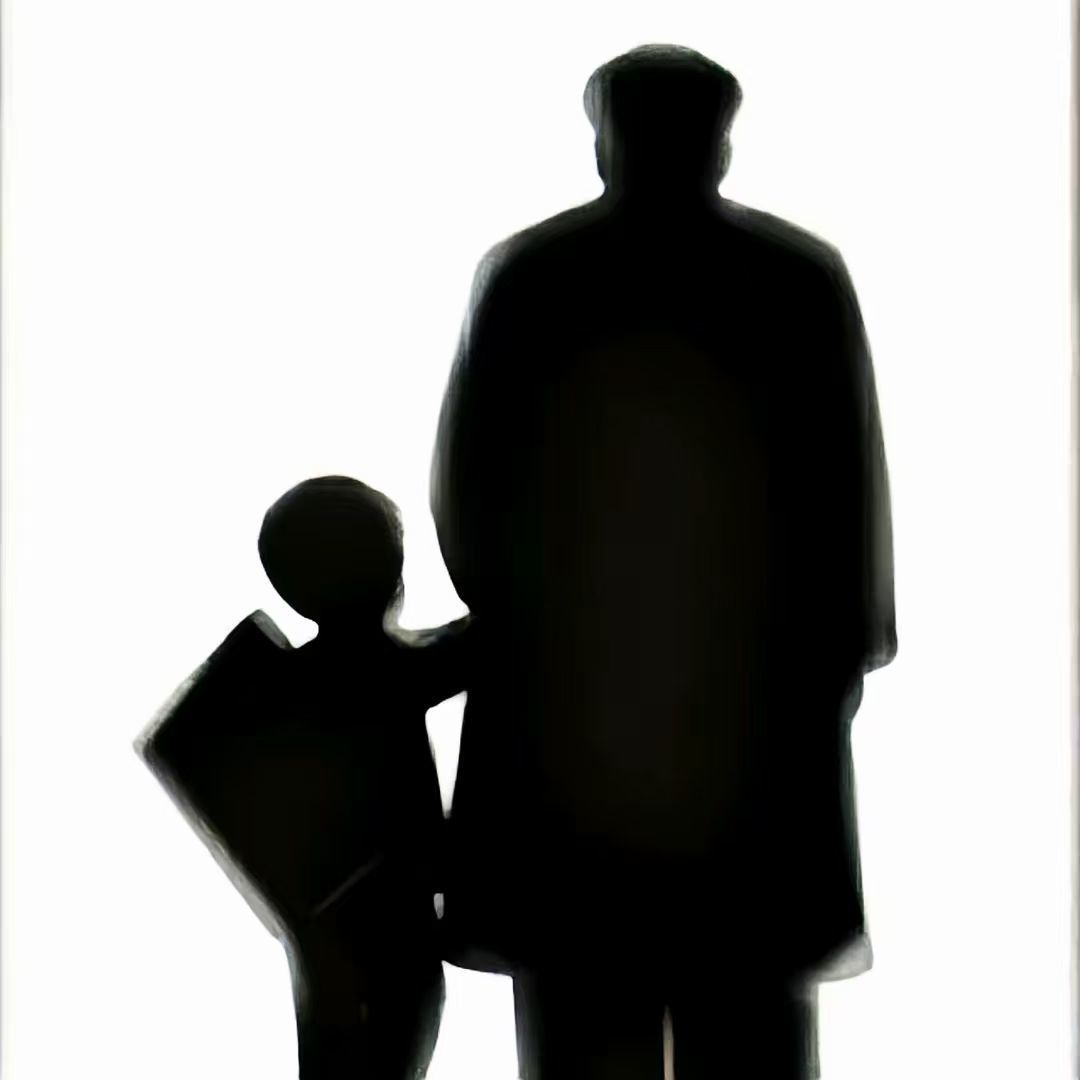
\includegraphics[width=1.0\textwidth]{Figs/teacher.jpeg}
    \caption{Mao and his son.}
\end{figure}
\end{document}